\chapter{Principios para la acción efectiva}
\label{cha:principios}

Por ahora, frente a la acelerada decadencia de nuestros vínculos políticos, creemos que es necesario crear un ecosistema de tecnologías cívicas para hacer efectivas las garantías jurídicas a las personas ciudadanas que, por sus condiciones particulares, no pueden tener acceso a la justicia o al gobierno. Este movimiento tiene que luchar por una cultura pirata, es decir, concentrada en hacer libres, abiertos y accesibles todos los recursos de los que dispone. De la misma manera, necesitamos desarrollar principios de política pública, de economía y de gobierno, que se vuelvan el sentido común de tanto de las planificadoras como de las estudiantes de las escuelas de negocios y de administración. En cierto sentido, se trata de desarrollar un nuevo pensamiento económico que haga frente a la visión neoclásica de entidades racionales y maximizadoras de utilidades. En cuanto a nuestra estrategia, nos reconocemos en una tensión entre la transparencia y la opacidad. Sabemos que el humor juega un papel fundamental en la conformación de un nuevo imaginario político. Hasta ahora, hemos pensado en algunos principios como parte de una visión efectiva de la táctica política progresista:

\section{Pragmatismo no es utilitarismo}
\label{sec:pragmatismo}

Muchas personas casadas con la Teoría crítica (marxismos, psicoanálisis, etcétera) satanizan la filosofía del hacer efectivo y eficiente. Nosotras pensamos que esta actitud de repudio a la estadística, a la optimización y a la eficacia son lo que nos ha valido tantas derrotas. Podemos pensar las cosas más románticas del mundo sobre la revolución, pero la realidad es que toda operación requiere un pensamiento estratégico, requiere instancias (es decir, medios concretos de ejecución, como el código en computación) y que no lograremos disputarle el sentido común al neoliberalismo, ni imaginar un más allá del Estado o del capitalismo si no pensamos que teoría, estrategia y práctica están interrelacionados y que no bastan buenas intenciones. Como lo señala Alinsky en su Tratado para radicales, las cuestiones morales no tienen ningún sentido frente a nuestros enemigos. Ahí mismo señala que la historia nos ha enseñado que primero se toma la acción y después se legitima.

\begin{figure}[htbp]
	\centering
	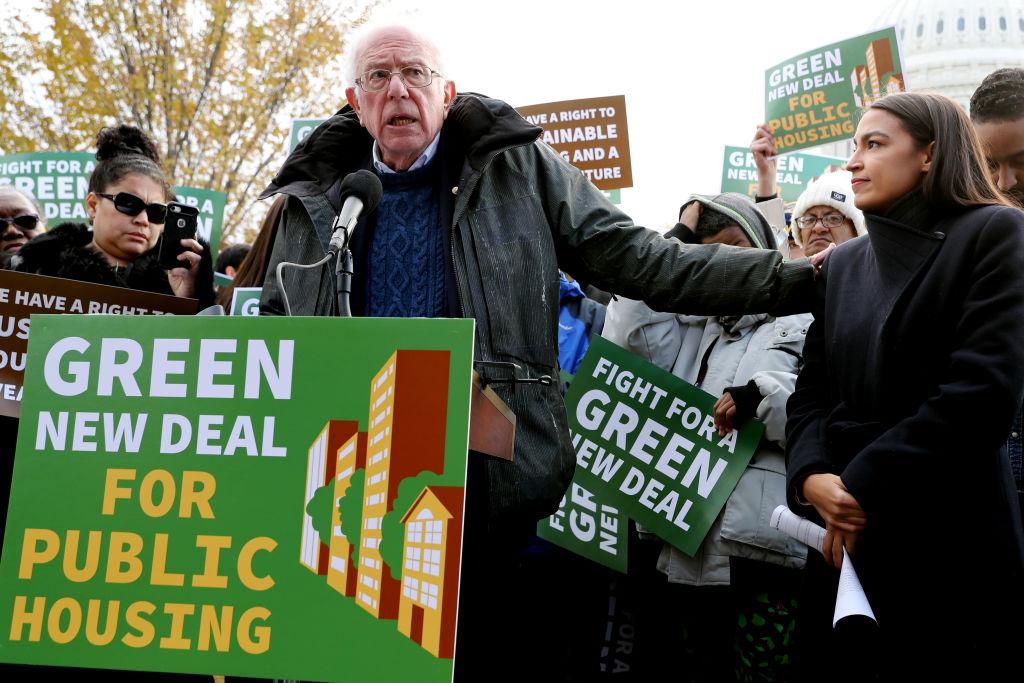
\includegraphics[width=0.9\linewidth]{green.jpg}
	\caption[Buen ejemplo de pragmatismo con sentido.]{Bernie Sanders, Alexandria Ocasio Cortés y el \emph{Green New Deal} son un buen ejemplo de pragmatismo con sentido.}
\end{figure}

\section{Interseccionalidad en la acción}
\label{sec:interseccionalidad}

Que todas nuestras acciones estén centradas en atender las condiciones estructurales de opresión a través de un movimiento emancipatorio que busque hacer frente de forma transversal a las diversas formas de violencia que padecen las personas. Para lograrlo, es necesario que entendamos cómo funciona el capitalismo hoy en día, en un contexto donde la fuerza de trabajo está totalmente precarizada, pulverizada y disuelta, en una época económica conocida como posfordismo, que consiste en una era donde la producción está profundamente ligada a la teoría de la información y de la computación. La interseccionalidad nos obliga a concentrarnos en desarrollar herramientas para comprender cómo funciona la explotación en sus distintas formas, por ejemplo, cómo se intersectan las violencias de género, racistas y de clase.

\begin{figure}[htbp]
	\centering
	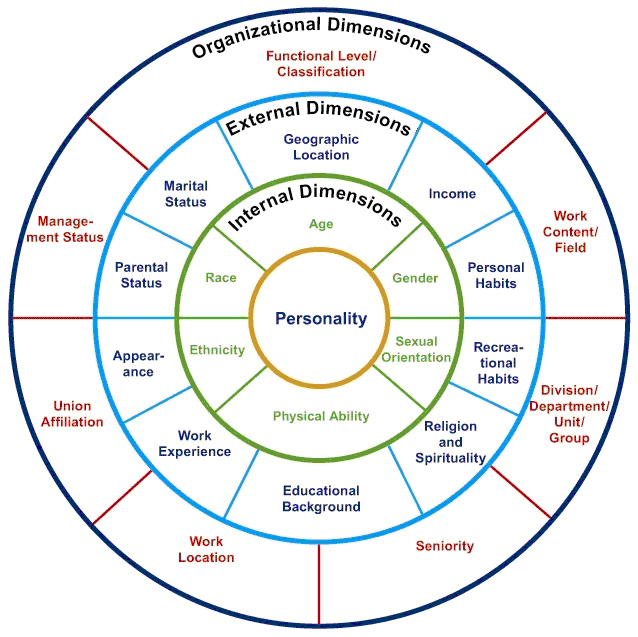
\includegraphics[width=\linewidth]{self-dimensions.png}
	\caption[Dimensiones de la personalidad.]{Dimensiones de la personalidad y factores de influencia.}
	\label{fig:dimensiones}
\end{figure}

\section{Transmisibilidad, o sea, hacernos accesibles}
\label{sec:transmisibilidad}

Si la ideología es el conjunto de significados culturales que nos hacen estar a favor o en contra de algo, necesitamos crear mecanismos de reconocimiento y traducción de estos significados para poder transformarlos. La mayoría de las personas no está realmente convencida de todo lo que cree y muchas veces lo cree más por ser receptora de un flujo de imágenes o de opiniones de gente con reputación social, que por su propio convencimiento. Ese es nuestro objetivo, ser capaces de comunicar a esas personas una visión comprensiva de la diferencia, de la otredad, de la dignidad del prójimo. Debemos hacer que nuestro discurso sea trans-ideológico, que pueda dialogar con distintas visiones reapropiándose y resignificando conceptos cooptados por conservadores y tradicionalistas (es decir, la derecha). Esta idea es parecida a lo que en ciencias sociales se conoce como intersubjetividad, que es la capacidad de las hablantes de crear significados comunes y compartidos que configuran su sentido común. Para lograr ser transmisibles, necesitamos más mercadotecnia para transmitir una cultura crítica y para comunicar el feminismo y la teoría crítica a gente que sabemos que podría accionar hacia una causa en particular, induciendo una disonancia cognitiva. Pensémoslo como si estas personas fueran \emph{swing voters} que tienen que elegir entre el sentido común neoliberal que las aliena o una visión crítica que las ayuda a reconocerse como personas con dignidad más allá de los códigos sociales. Pero no podemos hacer esto si no pensamos en los códigos de quienes nos escuchan. En el Corán, la \emph{taqiyya} o \emph{kitman} es el acto de disimular nuestras propias creencias en tiempos de persecución. Necesitamos disimular nuestras creencias y visibilizar mensajes seleccionado cuidadosamente para que logren insertarse en los flujos de deseo del capitalismo sin que el enemigo nos reconozca.

\begin{figure}[htbp]
	\centering
	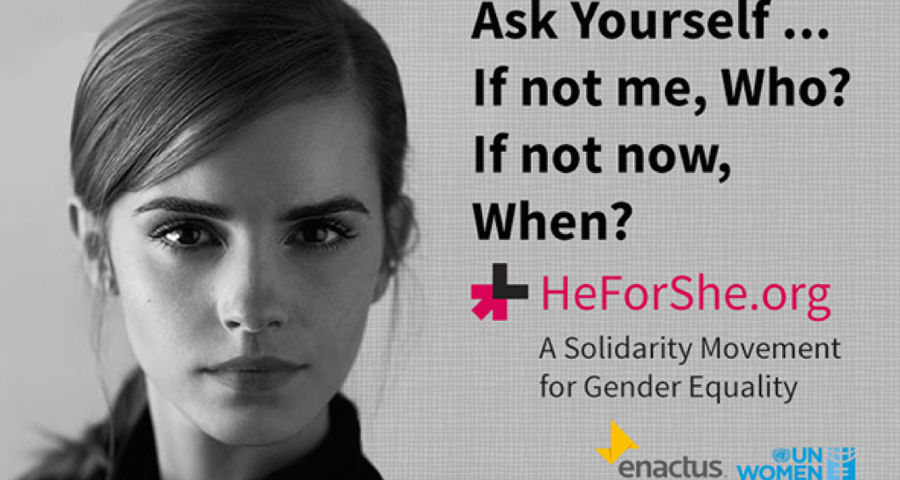
\includegraphics[width=\linewidth]{he4she.jpg}
	\caption[Emma Watson, vocera del \emph{He for She}.]{Emma Watson, vocera del \emph{He for She}, una forma de \emph{mainstreaming}.}
	\label{fig:he4she}
\end{figure}

\section{FLOSS y la bandera pirata}
\label{sec:FLOS}

En la jerga \emph{geek}, \emph{Free/Libre and Open Source Software} (FLOSS) es el tipo de software accesible a través de su código fuente. Esta filosofía es absolutamente necesaria para una práctica que permita el autogobierno de las personas y reduzca la dependencia del Estado y a los mecanismos tradicionales de gobierno, así como el poder de mercado de las corporaciones a través de las patentes. Nosotras añadiríamos \emph{Free/Libre and Open Source Culture} (FLOSC) para referirnos a un desarrollo en la cultura donde los procesos de creación de valor y de desarrollo de productos sean visibles y no ideológicos, es decir, que sirvan para que más gente pueda producir sus propios significados y sus propias estéticas y no para que sea utilizado para que la gente reproduzca un modelo de consumo (que es la función de la ideología). La cultura FLOS debe extenderse al espacio público, a la Academia, a los mercados (que hoy en día pertenecen a horribles lagartos que, a través de cinco empresas, controlan los flujos de distribución de mercancías y de imágenes en todo el planeta), a la educación y a todas las instituciones que reproducen el estado actual de las cosas. Esto significaría que el gobierno deje de operar empresas estatales y que más bien permita sus operaciones públicas, a través de certificaciones y procesos de descentralización, y no a través de la concesión a grandes monopolios transnacionales.\footnote{Entendemos, sin embargo, que hay problemas importantes cuando pensamos en proyectos que son intensivos en capital, como grandes obras de infraestructura o complejas investigaciones médicas. También se trata de acelerar los procesos de democratización y de FLOS dentro de la estructura de las corporaciones, que hoy en día, son reinos, con el todopoderoso CEO (\emph{Chief Executive Officer} o director general) gobierna sobre todos sus súbditos a través del salario.}

Respecto a la cuestión de las patentes, hay ideas muy interesantes como el \emph{copyleft} o el \emph{copyfair} que buscan reformular patentes y crear esquemas que fomenten cooperativas. Nosotras pensamos que este tipo de prácticas podrían servir en las licitaciones gubernamentales para generar leyes que obliguen a las instituciones públicas a tener procesos y patrones de cultura FLOS.

Otra idea con la que hemos coqueteado es con las etiquetas o \emph{labels} en inglés. Por ejemplo, una etiqueta \emph{Low tech} que certifique que ciertos productos desarrollados fueron diseñados como alternativas a la obsolescencia programada y con la posibilidad de intervenir sobre ellos. La idea de la etiqueta surge como una forma de crear un sistema de certificados que pueda competir con la lógica capitalista de producción de las grandes marcas, con la intención de desacelerar los ciclos de producción y consumo.

Algunas referencias interesantes para complementar este apartado:

\url{http://unenumerated.blogspot.com/2017/02/money-blockchains-and-social-scalability.html}

\url{http://unenumerated.blogspot.com/2006/11/wet-code-and-dry.html}

\begin{figure}[htbp]
	\centering
	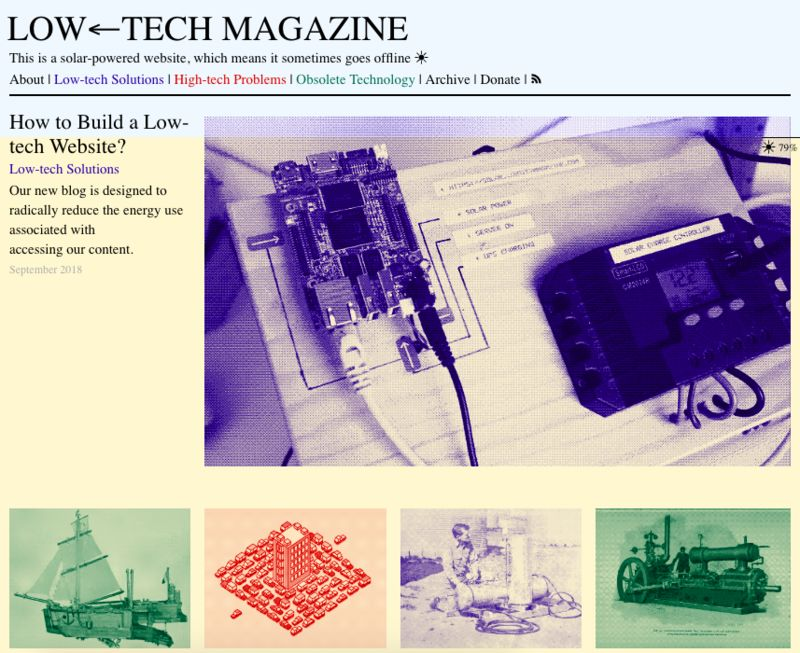
\includegraphics[width=.9\linewidth]{low-tech.jpeg}
	\caption[\emph{Low Tech Magazine}]{Imagen del sitio \emph{Low Tech Magazine}.}
	\label{fig:lowtech}
\end{figure}

\section{Queremos un mundo más allá de la economía capitalista}
\label{sec:mundo}

Algunas personas dicen que incluso si acabáramos con el capitalismo como forma de explotación, todavía habría que pensar en cómo ir más allá de relaciones sociales mediadas por abstracciones como la moneda. ¿Por qué? Cada vez presenciamos cómo hasta la última esfera de la vida está sujeta a la regulación, a la medición y a la cuantificación. Esto nos impide vivir sin considerarnos a través de márgenes de utilidad y hace que nos sigamos mirando las unas a las otras, al menos parcialmente, como objetos de interés. La cibernética es la ciencia y arte del control que cuantifica cada vez más toda experiencia de vivir en \emph{clicks}, en \emph{shares}, en \emph{likes}, y esto no hace sino aumentar el deseo de enjuiciarnos cada vez más. Una posible solución está en pensar que las tecnologías que desarrollemos para crear un Estado más justo también tienen que preguntarse cómo haremos para generar más vínculos, más encuentros donde las personas puedan hablar, escucharse y establecer vínculos más allá de la pertenencia a una tribu identitaria o a cualquier grupo de interés. Creemos que el verdadero problema de la tecnología es su desarrollo capitalista, que desorganiza a las personas para volverse cada vez más necesaria.

Para lograrlo, podemos valernos de investigaciones como \emph{Nudge economy}, parte de la economía de la conducta que analiza el diseño de incentivos que conducen a la gente a tomar decisiones, es decir, la disposición económica de los objetos a las personas. En este campo es también posible vincular la experiencia de usuario o UX (\emph{user experience}) para hacer interfaces más accesibles e incluso más comunitarias.

\begin{figure}[htbp]
	\centering
	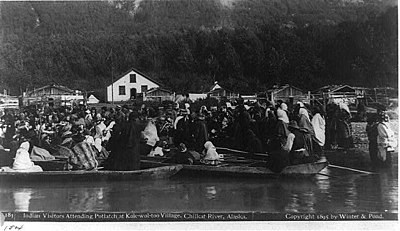
\includegraphics[width=\linewidth]{potlatch.jpg}
	\caption[\emph{Potlatch}.]{El \emph{potlatch}, concepto clave en la economía del don de Marcell Mauss, es un ritual de los pueblos aborígenes de la costa del Pacífico en el noroeste de Norteamérica, tanto en los Estados Unidos como en la provincia de la Columbia Británica de Canadá. EE.UU.}
	\todo[inline]{Corregir el brillo y contraste de la imagen para que se pueda ver con más claridad.}
	\label{fig:potlatch}
\end{figure}

\section{Luchemos por estar en los canales masivos}
\label{sec:luchemos}

El algoritmo del capitalismo funciona implantándonos deseos de consumir y de cumplir ciertos códigos sociales que siempre tienden al individualismo y a la mercantilización de las otras personas. No creemos en la falsa dicotomía entre luchas locales y globales, creemos que hoy en día, toda forma de activismo es una cierta tecnopolítica. Es decir, que nuestras prácticas contienen cierta posición estratégica sobre el uso de los recursos en decisiones tan básicas como usar manuales de \emph{zero waste} en eventos públicos y hacer campañas para hacerlo una moda. Si realmente queremos hacer algo efectivo, tenemos que crear un \emph{mainstream} o corriente mayoritaria que permita unir distintos proyectos que luchan por la emancipación así como los ingleses tienen BBC como distintivo de su identidad y de su cultura.

El trueque, el \emph{freeganism} o los bancos de tiempo son estrategias de resistencia que por sí solas, aisladas en contextos locales, de micropolítica, no pueden hacer nada para ganarle a los millones de dólares que la industria de la comida rápida invierte en hacernos desear el azúcar, las grasas y cualquiera de esas sustancias que nos restan salud. Sin embargo, combinadas en una campaña masiva y consolidando audiencias que puedan encontrar alternativas sistémicas como salud pública y comedores comunitarios, empezaremos a tener victorias reales. Es decir, hay que crear flujos alternativos a la cultura de masas que tengan aspiren a una plataforma común de organización, para hacer publicidad no a un proyecto de bajo impacto en particular, sino a una alternativa sistémica y escalable. Para nosotras, Wikipolítica fue la muestra de que tenemos la capacidad de hacer funcionar una maquina capaz de hacer campanas de mercadotecnia con alcance nacional que lleguen a diferentes segmentos e incluso lleguen a medios masivos internacionales.

\section{La crítica debe enfocarse en las tecnologías que producen la opresión}
\label{sec:critica}

Nuestro discurso debería ser interseccional e incluir en su agenda un conjunto de propuestas sistemáticas en torno a cada lucha particular. En la dinámica actual del capitalismo, hacer uso de las marcas puede darle más poder a la lucha. Necesitamos crear una red para consolidar, para entablar puentes de colaboración de saberes técnicos. Es importante mencionar que en la cooperación técnica se pueden hacer progresos discursivos paralelos, una identidad mínima interseccional, un vínculo común de articulación para la comunicación estratégica de una red de círculos que construyan una plataforma con procesos y patrones en común para incentivar la participación política.

Se nos ocurre que incluso sería buena idea hacer campamentos de inteligencia colectiva. Estos deberán operar a través de la escucha y plantear preguntas de empatía: ¿cómo se sienten hoy? ¿Cuál fue tu logro más importante de esta semana? ¿Qué problemas hay en la organización? ¿Qué respuestas podemos crear desde nuestra posición para solucionar el problema? ¿Cómo se sintieron con esta dinámica? Nos imaginamos talleres diversos, como educación popular, herramientas de mapeo, el buen trato como estrategia de lucha, participación ciudadana, herramientas filosóficas, lluvia de ideas y dinámicas de inteligencia colectiva para una cartografía de controversias.

Hoy en día es posible desarrollar la economía social para tratar de enlazar distintos proyectos de resistencia, basados en estructuras de micro mecenazgo. El horizonte educativo podría ser una cruzada contra el analfabetismo digital, con la intención de que todas las personas puedan navegar en la complejidad de la era de la información.
